\documentclass[11pt,open=any,oneside,parskip=half]{scrbook}

\usepackage[ngerman]{babel}
\usepackage{fontspec}
\usepackage{geometry}
\usepackage{microtype}
\usepackage{graphicx}
\usepackage{eso-pic}
\usepackage{tikz}
\usetikzlibrary{calc}
\usepackage{booktabs}
\usepackage{longtable}
\usepackage{array}
\usepackage{tabularx}
\usepackage{amsmath}
\usepackage{multicol}
\usepackage{enumitem}
\usepackage{etoolbox}
\usepackage{xcolor}
\usepackage{hyperref}
\usepackage{cleveref}
\crefname{chapter}{Kapitel}{Kapitel}
\Crefname{chapter}{Kapitel}{Kapitel}
\crefname{appendix}{Anhang}{Anhänge}
\Crefname{appendix}{Anhang}{Anhänge}
\usepackage{pdfpages}
\usepackage{scrlayer-scrpage}
\usepackage{makeidx}
\usepackage{amstext}
\makeindex

\geometry{left=3cm,right=3cm,top=3.5cm,bottom=3.5cm}
\setcounter{secnumdepth}{0}
\setcounter{tocdepth}{2}
\setlength{\columnsep}{20pt}
\setlength{\multicolsep}{0pt}
\setlist[description]{style=nextline,leftmargin=0pt,font=\normalfont\small}
\raggedcolumns

\setmainfont{EBGaramond-Regular.ttf}[
  Path=assets/fonts/,
  BoldFont=EBGaramond-Bold.ttf,
  ItalicFont=EBGaramond-Italic.ttf,
  BoldItalicFont=EBGaramond-BoldItalic.ttf
]
\setsansfont{Metamorphous-Regular.ttf}[
  Path=assets/fonts/,
  BoldFont=Metamorphous-Regular.ttf,
  BoldFeatures={FakeBold=1.5},
  ItalicFont=Metamorphous-Regular.ttf,
  ItalicFeatures={FakeSlant=0.2}
]
\newfontfamily\displayfont{Metamorphous-Regular.ttf}[
  Path=assets/fonts/,
  ItalicFont=Metamorphous-Regular.ttf,
  ItalicFeatures={FakeSlant=0.2},
  SlantedFont=Metamorphous-Regular.ttf,
  SlantedFeatures={FakeSlant=0.2},
  BoldFont=Metamorphous-Regular.ttf,
  BoldFeatures={FakeBold=1.5}
]
\setmonofont{Oxanium-Regular.ttf}[
  Path=assets/fonts/,
  BoldFont=Oxanium-Bold.ttf
]

\definecolor{primarytext}{RGB}{20,18,17}
\definecolor{examplecolor}{RGB}{34,94,56}
\definecolor{quotecolor}{RGB}{140,52,28}
\definecolor{linkcolor}{RGB}{143,49,20}
\definecolor{ruleaccent}{RGB}{84,33,20}
\color{primarytext}
\newcommand{\tirakanversion}{0.3.0}


\hypersetup{
  colorlinks=true,
  linkcolor=linkcolor,
  urlcolor=linkcolor,
  pdftitle={Tirakans Reiche Regelbuch},
  pdfauthor={OpenAI Codex},
  pdfsubject={Version \tirakanversion}
}

\AddToShipoutPictureBG{%
  \AtPageLowerLeft{%
    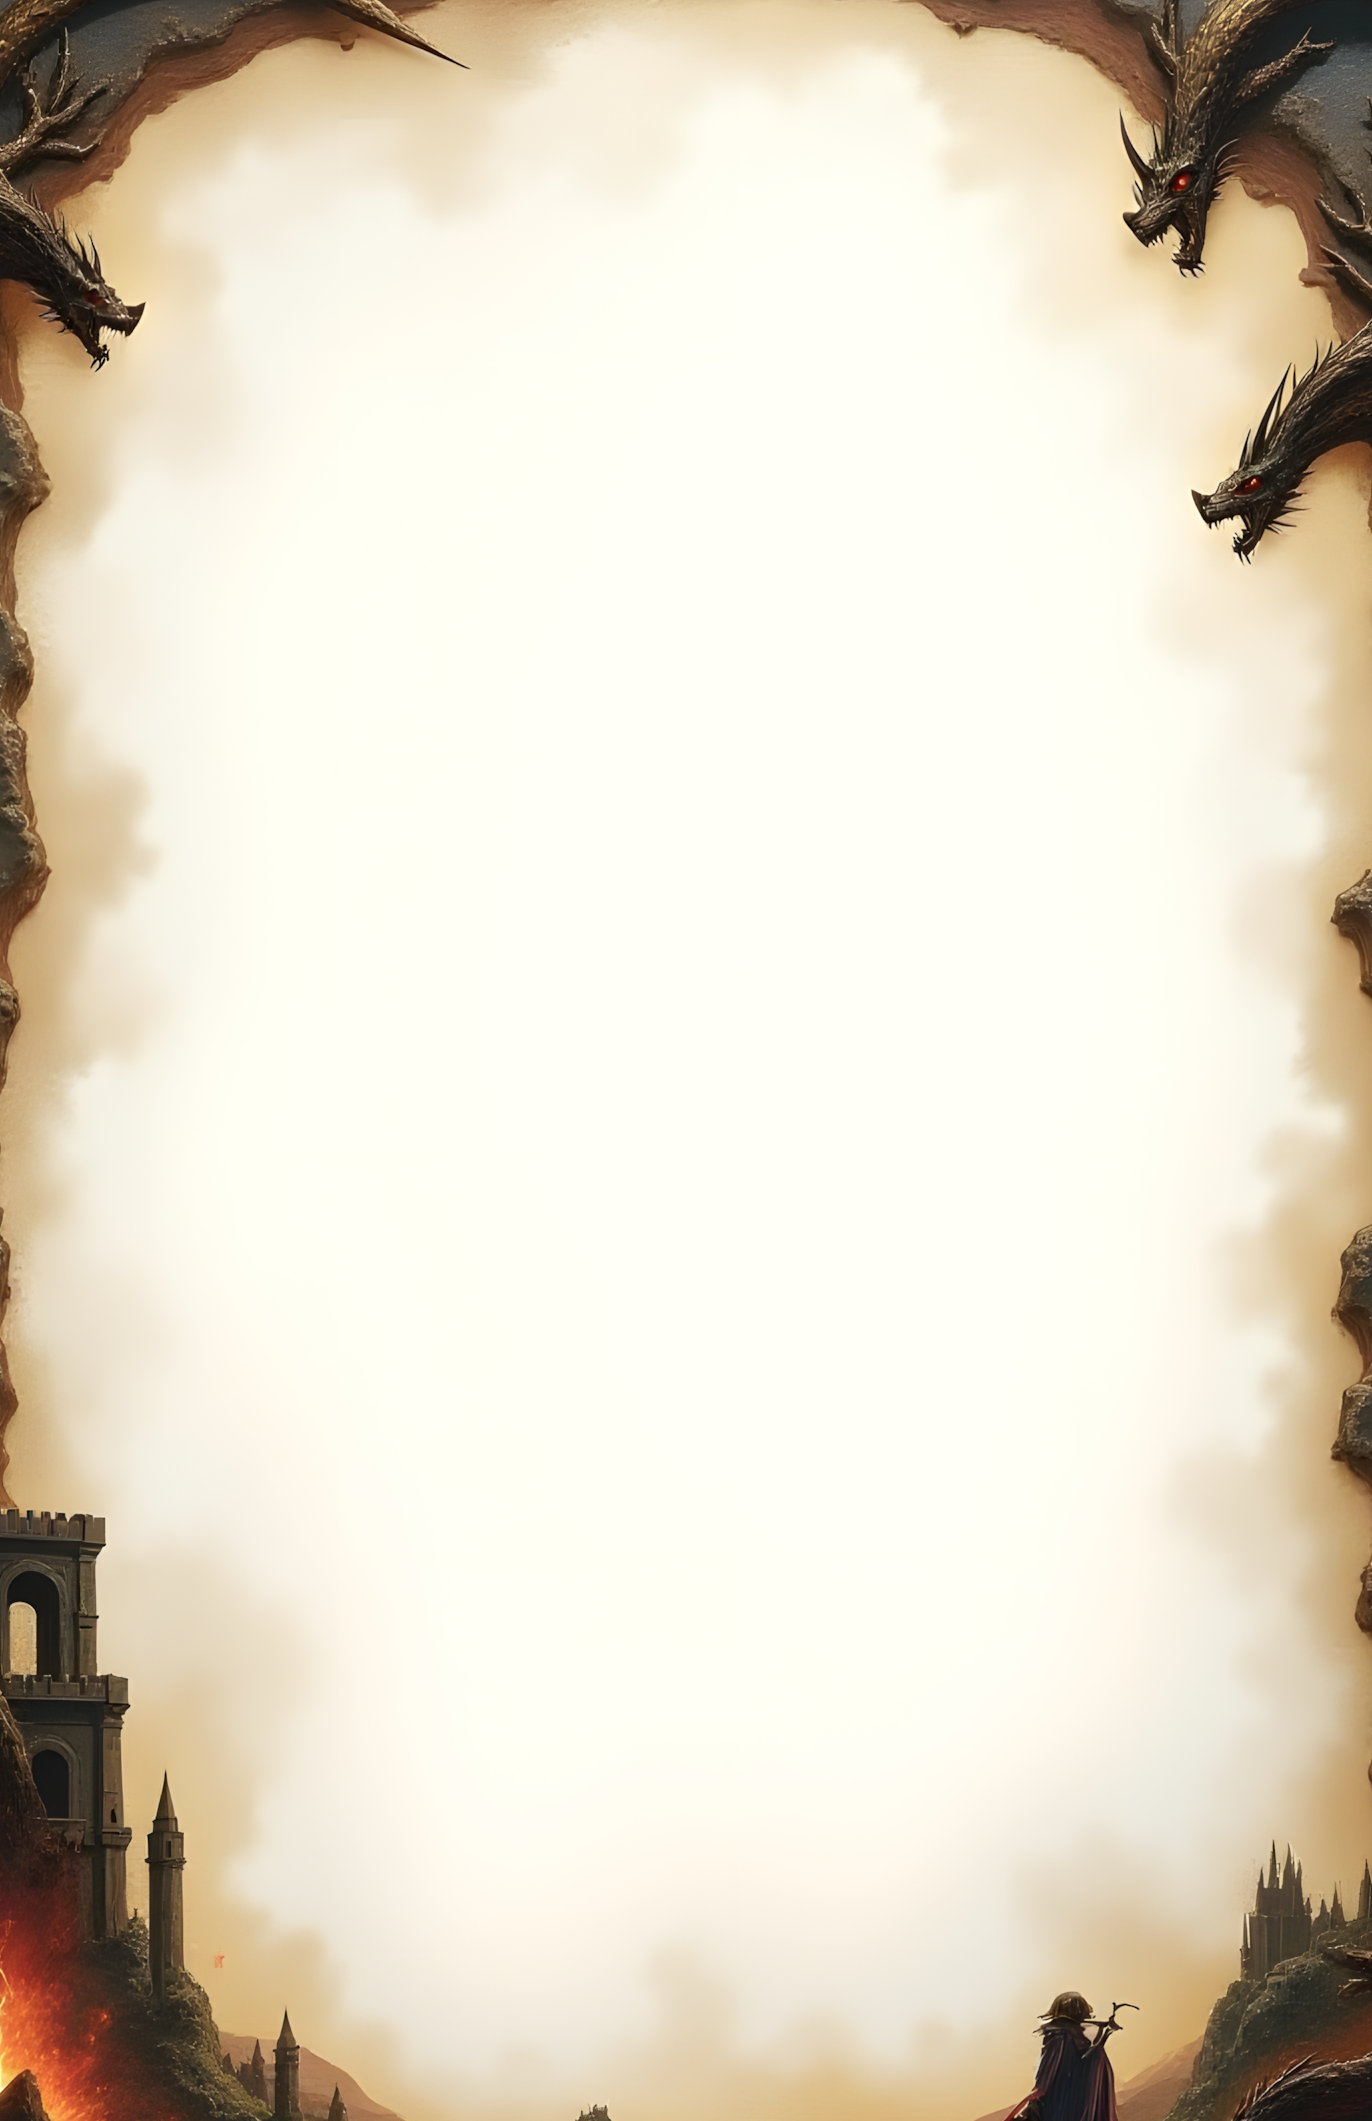
\includegraphics[width=\paperwidth,height=\paperheight]{assets/images/tirakan-background.png}%
  }%
}

\clearpairofpagestyles
\ihead{}
\ohead{}
\cfoot{\displayfont\thepage}

\newcommand{\booktitle}{Tirakans Reiche}
\newcommand{\booksubtitle}{Freies Dark-Fantasy-Rollenspiel}
\newcommand{\trans}[1]{#1}

\newcommand{\chapterimage}[1]{assets/images/chapters/tirakan-#1.png}

\let\origchapterlinesformat\chapterlinesformat
\renewcommand*{\chapterlinesformat}[3]{}
\makeatletter
\newcommand{\printtoc}{\@starttoc{toc}}
\newcommand{\renderchapterpage}[2]{%
  \thispagestyle{empty}%
  \begin{tikzpicture}[remember picture,overlay]
    \path[use as bounding box] (current page.south west) rectangle (current page.north east);
    \node[inner sep=0pt] at (current page.center) {\includegraphics[width=\paperwidth,height=\paperheight]{\chapterimage{#2}}};
    \fill[black, opacity=0.42] (current page.south west) rectangle (current page.north east);
    \node[
      anchor=north west,
      text=white,
      font=\displayfont\fontsize{52pt}{66pt}\selectfont,
      inner sep=10pt
    ] at ([xshift=1.5cm,yshift=-1.5cm]current page.north west) {\thechapter};
    \node[
      anchor=south east,
      text=white,
      align=right,
      font=\displayfont\fontsize{40pt}{50pt}\selectfont,
      text width=0.82\paperwidth
    ] at ([xshift=-1.5cm,yshift=1.5cm]current page.south east) {#1};
  \end{tikzpicture}%
}
\newcommand{\worldchapter}[3][]{%
  \if@openright\cleardoublepage\else\clearpage\fi
  \refstepcounter{chapter}%
  \phantomsection
  \if\relax\detokenize{#1}\relax
    \addcontentsline{toc}{chapter}{\protect\numberline{\thechapter}#2}%
    \chaptermark{#2}%
  \else
    \addcontentsline{toc}{chapter}{\protect\numberline{\thechapter}#1}%
    \chaptermark{#1}%
  \fi
  \renderchapterpage{#2}{#3}%
  \clearpage
}
\makeatother

\newenvironment{ruleexample}[1][Beispiel]
{\par\smallskip\noindent\color{ruleaccent}\textbf{#1. }\itshape}
{\par\smallskip}

\newenvironment{pexample}[1][]
{
  \color{examplecolor}
  \ifstrempty{#1}{}{
    \par\addvspace{0.5em}
    \noindent\textbf{#1}\par\nopagebreak
    \addvspace{0.1em}
  }
}
{
  \par\addvspace{1em}
}

\newcommand{\pquoteauthor}{}
\newenvironment{pquote}[1]
{
  \renewcommand{\pquoteauthor}{#1}
  \begin{flushright}
  \color{quotecolor}
  \slshape
}
{
  \\ \medskip
  \upshape\textit{\pquoteauthor}
  \end{flushright}
}

\newcommand{\abstammungspielwertebox}[3]{%
  \medskip
  \noindent\begin{tikzpicture}
    \node[
      draw=ruleaccent!70,
      fill=ruleaccent!6,
      rounded corners=4pt,
      line width=0.6pt,
      inner xsep=10pt,
      inner ysep=9pt,
      text width=\dimexpr\columnwidth-20pt\relax,
      align=left
    ] (spielwertebox) {%
      \vspace{0.25\baselineskip}%
      \setlength{\parskip}{0pt}%
      \setlength{\parindent}{0pt}%
      \raggedright
      \textbf{Vorteil:} #1\par
      \smallskip
      \textbf{Verwundbarkeit:} #2\par
      \smallskip
      \textbf{Fertigkeiten:} #3%
    };
  \end{tikzpicture}
  \medskip
}

\newcommand{\wegespielwertebox}[4]{%
  \medskip
  \noindent\begin{tikzpicture}
    \node[
      draw=ruleaccent!70,
      fill=ruleaccent!6,
      rounded corners=4pt,
      line width=0.6pt,
      inner xsep=10pt,
      inner ysep=9pt,
      text width=\dimexpr\columnwidth-20pt\relax,
      align=left
    ] (spielwertebox) {%
      \vspace{0.25\baselineskip}%
      \setlength{\parskip}{0pt}%
      \setlength{\parindent}{0pt}%
      \raggedright
      \textbf{Vorteil:} #1\par
      \smallskip
      \textbf{Verwundbarkeit:} #2\par
      \smallskip
      \textbf{Wegfacette:} #3\par
      \smallskip
      \textbf{Fertigkeiten:} #4%
    };
  \end{tikzpicture}
  \medskip
}

\newcommand{\praegungsfertigkeiten}[1]{%
  \noindent\textbf{Fertigkeiten:} #1\par
  \medskip
}

\newcommand{\bindungspielwertebox}[2]{%
  \medskip
  \noindent\begin{tikzpicture}
    \node[
      draw=ruleaccent!70,
      fill=ruleaccent!6,
      rounded corners=4pt,
      line width=0.6pt,
      inner xsep=10pt,
      inner ysep=9pt,
      text width=\dimexpr\columnwidth-20pt\relax,
      align=left
    ] (spielwertebox) {%
      \vspace{0.25\baselineskip}%
      \setlength{\parskip}{0pt}%
      \setlength{\parindent}{0pt}%
      \raggedright
      \textbf{Vorteil:} #1\par
      \smallskip
      \textbf{Verwundbarkeit:} #2%
    };
  \end{tikzpicture}
  \medskip
}

\newcommand{\malspielwertebox}[2]{%
  \medskip
  \noindent\begin{tikzpicture}
    \node[
      draw=ruleaccent!70,
      fill=ruleaccent!6,
      rounded corners=4pt,
      line width=0.6pt,
      inner xsep=10pt,
      inner ysep=9pt,
      text width=\dimexpr\columnwidth-20pt\relax,
      align=left
    ] (spielwertebox) {%
      \vspace{0.25\baselineskip}%
      \setlength{\parskip}{0pt}%
      \setlength{\parindent}{0pt}%
      \raggedright
      \textbf{Vorteil:} #1\par
      \smallskip
      \textbf{Verwundbarkeit:} #2%
    };
  \end{tikzpicture}
  \medskip
}

\newcommand{\spelltag}[1]{%
  \tikz[baseline=(spelltag.base)]\node[
    draw=ruleaccent!35,
    fill=ruleaccent!6,
    rounded corners=3pt,
    line width=0.5pt,
    inner xsep=5pt,
    inner ysep=1.5pt,
    text=primarytext!70,
    font=\sffamily\fontsize{7.5pt}{8.5pt}\selectfont
  ] (spelltag) {#1};%
}

\newcommand{\spellheader}[3]{%
  \par\nobreak
  \vspace{-0.45\baselineskip}%
  {\noindent\small
    \spelltag{#1}\hspace{0.35em}%
    \spelltag{#2}%
    \ifstrequal{#3}{1 Kampfhandlung}{}{%
      \hspace{0.35em}\spelltag{Ritual}%
    }%
    \par
  }%
  \vspace{0.35\baselineskip}%
}

\newcommand{\spellinfobox}[7]{%
  \noindent\begin{tikzpicture}
    \node[
      draw=ruleaccent!70,
      fill=ruleaccent!6,
      rounded corners=4pt,
      line width=0.6pt,
      inner xsep=10pt,
      inner ysep=8pt,
      text width=\dimexpr\columnwidth-20pt\relax,
      align=left
    ] {%
      \setlength{\parskip}{0pt}%
      \setlength{\parindent}{0pt}%
      \footnotesize
      \renewcommand{\arraystretch}{1.05}%
      \begin{tabular*}{\linewidth}{@{\extracolsep{\fill}}p{0.47\linewidth}p{0.47\linewidth}@{}}
        \textbf{ZP:} #1 & \textbf{Arkana:} #2 \\
        \textbf{Reichweite:} #3 & \textbf{Dauer:} #4 \\
        \textbf{Form:} #5 & \textbf{Wirken:} #6 \\
        \multicolumn{2}{@{}p{\linewidth}@{}}{\textbf{Konzentration:} #7} \\
      \end{tabular*}%
    };
  \end{tikzpicture}
  \vspace{0.45\baselineskip}%
}

\begin{document}

\begin{titlepage}
  \begin{tikzpicture}[remember picture,overlay]
    \path[use as bounding box] (current page.south west) rectangle (current page.north east);
    \node[inner sep=0pt] at (current page.center) {\includegraphics[width=\paperwidth,height=\paperheight]{assets/images/tirakan-title.png}};
    \fill[black, opacity=0.42] (current page.south west) rectangle (current page.north east);
    \coordinate (titlepos) at ([yshift=-5.8cm]current page.north);
    \node[
      text=white,
      font=\displayfont\bfseries\fontsize{42}{48}\selectfont,
      align=center
    ] at ([yshift=0.85cm]titlepos) {Tirakans};
    \begin{scope}[white, line width=0.8pt]
      \coordinate (linecenter) at (titlepos);
      \draw ($(linecenter)+(-9em,0)$) -- ($(linecenter)+(-1.5em,0)$);
      \draw ($(linecenter)+(9em,0)$) -- ($(linecenter)+(1.5em,0)$);
      \node[rotate=45,draw,inner sep=2.5pt] at (linecenter) {};
    \end{scope}
    \node[
      text=white,
      font=\displayfont\bfseries\fontsize{42}{48}\selectfont,
      align=center
    ] at ([yshift=-0.85cm]linecenter) {Reiche};
    \node[
      text=white,
      font=\displayfont\Large\itshape,
      text width=0.7\textwidth,
      align=center
    ] at ([yshift=-2.8cm]linecenter) {\booksubtitle};
    \node[
      text=white,
      font=\displayfont\large\selectfont,
      align=center
    ] at ([yshift=-4.0cm]linecenter) {Version \tirakanversion};
  \end{tikzpicture}
\end{titlepage}

\frontmatter
\pagestyle{empty}
\addchap*{Inhalt}
\begin{multicols*}{2}
  \setlength{\parskip}{0pt}
  \printtoc
\end{multicols*}

\mainmatter
\pagestyle{scrheadings}

\include{chapters/vorwort}
\worldchapter{Die Regeln}{game-rules}
\label{ch:game-rules}

\begin{multicols*}{2}

Obwohl die Spielleiterin die Bösen steuert, steht sie eigentlich auf der Seite der Helden.
Spieler und Spielleiterin begeben sich zusammen auf eine fantastische Reise, bei der die Erzählung im Vordergrund steht.

Die Spieler steuern ihre \textbf{Charaktere} in dieser fiktiven Welt, und handeln in ihrem Namen.
Die Fähigkeiten eines Charakters, ihr Hab und Gut, ihre Stärken und Schwächen werden auf dem \textbf{Charakterbogen} niedergeschrieben.
Du als Spieler beschreibst der Spielleiterin das Handeln deines Charakters.
Möglicherweise erfordert die Handlung deines Charakters eine \textbf{Probe}, einen Test auf ein bestimmtes \textbf{Attribut}, bei dem passende \textbf{Fertigkeiten} zusätzliche Vorteile geben können.

Diese Proben sind der Kern des Spiels.
Es ist die Grundmechanik, um über den Erfolg oder das Misslingen einer Handlung zu bestimmen.

\section{Die Probe}\label{sec:die-probe}

Die Probe\index{Probe} ist der zentrale Bestandteil der Regeln.
Wenn eine Situation einen ungewissen Ausgang hat, wird eine Probe verwendet, um den Ausgang der Situation zu bestimmen.
Tirakans Reiche benutzt für alle Proben einen hundertseitigen Würfel, einen \textbf{W100}.
In der Regel werden zwei zehnseitige Würfel (\textbf{W10}) geworfen, wobei einer der Würfel die Zehnerstelle und der andere die Einerstelle des Wurfes darstellen.
Ein Ergebnis von \textbf{00} bedeutet 100.

Ob Erkundung, soziale Spannung, Verfolgung, Ritual oder Kampf: Wenn der Ausgang unsicher ist und Konsequenzen hat, wird eine Probe abgelegt.

Die Regeln legen besonderen Wert auf den Ausgang der Probe. Es ist nicht einfach nur ein geschafft oder nicht geschafft, es wird besonderen Wert auf die \textbf{Konsequenzen} einer Probe gelegt. Ob im alltäglichen, im Handwerk oder beim Ausüben von Magie, jede Probe hat Folgen für die Situation oder den Charakter.

\subsection{Zielwert}\label{subsec:zielwert}

Eine Probe wird immer auf genau ein \textbf{Attribut}\index{Attribut} geworfen.
Die Spielleiterin bestimmt das passende Attribut für die Situation, wenn die Regeln nicht etwas anderes vorsehen.
Zu den Attributen zählen \textbf{Geist}, \textbf{Wille}, \textbf{Instinkt}, \textbf{Geschick}, \textbf{Körper}, \textbf{Erscheinung}, \textbf{Gabe} und \textbf{Wahrnehmung}.


Dieser \textbf{Zielwert}\index{Zielwert} muss unterschritten werden, damit die Probe erfolgreich ist. Dieser Zielwert ist gestaffelt nach dem Rang, den der Charakter in dem Attribut hat:\\

\begin{tabular}{ll}
    \toprule
    \textbf{Attribut}  & \textbf{Zielwert}\\
    \midrule
    \textbf{0}        & 30 \\
    \textbf{1}        & 45 \\
    \textbf{2}        & 60 \\
    \textbf{3}        & 75 \\
    \textbf{4}        & 90 \\
    \bottomrule
\end{tabular}

Der Zielwert wird immer auf 5 bis 95 begrenzt.
Eine Probe gelingt, wenn der Wurf kleiner als der Zielwert ist.

\subsection{Fertigkeit}\label{subsec:probe-fertigkeit}

Besitzt der Charakter eine passende Fertigkeit, die er in der Situation einsetzen kann, so gelten die Vorteile der Fertigkeit. Fertigkeiten sind ausführlich in \cref{sec:fertigkeiten} beschrieben. Fertigkeiten entscheiden, ob eine Handlung fachgerecht möglich ist und welche Rangvorteile gelten, verändern den Zielwert aber nicht.

\begin{tabularx}{\linewidth}{lX}
    \toprule
    \textbf{Fertigkeit}  & \textbf{Effekt}\\
    \midrule
    \textbf{0 Improvisiert}        & Bei Misslingen der Probe wird die Konsequenzstufe um eins erhöht.\\
    \textbf{1 Geübt}        &  Knapp gescheiterte Proben zählen als Stillstand und nicht als geringe Konsequenz.\\
    \textbf{2 Erfahren}        & Einmal pro Szene darf eine Probe neu gewürfelt werden, das neue Ergebnis zählt. \\
    \textbf{3 Meisterlich}        & Wenn die Probe gelingt, wird die Ergebnisstufe um eins angehoben.  \\
    \textbf{4 Legendär}        & Einmal pro Szene darf das Ergebnis einer Probe vollständig ignoriert werden. \\
    \bottomrule
\end{tabularx}

Die Stufen der Fertigkeiten gelten kumulativ. Das bedeutet, dass ein Charakter mit einem Rang von 3 in einer Fertigkeit bei einem Wurf auch die Boni der Ränge 1 und 2 bekommt.

\subsection{Schwierigkeit}

Eine Probe kann erschwert sein, wenn sie unter schwierigen Bedingungen ausgeführt wird.
Die Spielleiterin legt hier einen Malus fest, der vor dem Wurf auf den Zielwert angerechnet wird, bevor geworfen wird.

\begin{itemize}[leftmargin=*]
\item \textbf{Leicht}: +20
\item \textbf{Standard}: +0
\item \textbf{Schwer}: -20
\item \textbf{Extrem}: -40
\end{itemize}

\subsection{Ablauf einer Probe}

\begin{enumerate}[leftmargin=*]
\item Der Spieler beschreibt Absicht und Vorgehen.
\item Die Spielleiterin bestimmt das passende Attribut und legt fest, ob eine passende Fertigkeit die Handlung stützt, einschränkt oder improvisiert werden muss.
\item Alle Modifikatoren werden zusammengerechnet.
\item Es wird 1W100 gewürfelt.
\item Ergebnisstufe, unmittelbare Wirkung und Konsequenz werden sofort abgehandelt.
\end{enumerate}

\subsection{Ergebnisstufe}

Das Resultat der Probe ergibt die Ergebnisstufe.
Ist der geworfene Wert bis zu 10 Punkte vom Zielwert entfernt, so ist die Probe knapp gelungen oder misslungen.
Weicht er mehr als 30 Punkte ab, so handelt es sich um einen starken Erfolg oder schweren Fehlschlag.
Ein Wurf von 01--05 ist immer ein kritischer Erfolg, alles von 96--100 ist immer ein katastrophales Scheitern.

\begin{tabular}{ll}
    \toprule
    \textbf{Ergebnisstufe}            & \textbf{Wurf}          \\
    \midrule
    \textbf{Kritischer Erfolg}        & 01--05   \\
    \textbf{Starker Erfolg}           & Marge 30+        \\
    \textbf{Sauberer Erfolg}          & Marge 10--29     \\
    \textbf{Knapp geschafft}          & Marge 0--9       \\
    \textbf{Knapp gescheitert}        & Marge 1--9   \\
    \textbf{Klar gescheitert}         & Marge 10--29 \\
    \textbf{Schwer gescheitert}       & Marge 30+    \\
    \textbf{Katastrophal gescheitert} & 96--00    \\
    \bottomrule
\end{tabular}

\subsection{Konsequenzen}\label{sec:konsequenzen}

Jede misslungene Probe kann zu \textbf{Konsequenzen}\index{Konsequenz} führen, die über die eigentliche Intention der Probe hinaus gehen.
Konsequenzen werden in drei Kategorien eingeteilt und haben unterschiedliche Folgen.
Diese werden von der Spielleiterin festgelegt.

\begin{itemize}[leftmargin=*]
\item \textbf{Gering}: kurze Verzögerung, kleiner Verlust, kurze Irritation.
\item \textbf{Ernst}: Wunde, deutlicher Verlust, Eskalation, schlechtere Position.
\item \textbf{Kritisch}: schwere Wunde, Zielverschiebung, massiver Kollateralschaden, bleibende Folge.
\end{itemize}

In der Regel führt eine bestimmte Ergebnisstufe immer zu einer bestimmten Klasse an Konsequenzen, dies kann natürlich je nach Situation von der Spielleiterin verändert werden.

\begin{itemize}[leftmargin=*]
\item Knapp gescheitert \textrightarrow{} Gering
\item Klar gescheitert \textrightarrow{} Ernst
\item Schwer oder katastrophal gescheitert \textrightarrow{} Kritisch
\item Knapp geschafft in einer verzweifelten Lage \textrightarrow{} Erfolg mit geringer Konsequenz
\end{itemize}

\subsection{Gegenproben}\label{sec:gegenproben}

Wenn zwei Seiten direkt gegeneinander handeln, würfeln beide gegen ihren eigenen Zielwert.

\begin{itemize}[leftmargin=*]
\item Eine Seite gelingt, die andere scheitert: Die erfolgreiche Seite gewinnt.
\item Beide gelingen: Die höhere Erfolgs-Marge gewinnt.
\item Beide scheitern mit 10+ Differenz: die geringere Fehlmarge bekommt die \textbf{Oberhand}\index{Oberhand}.
\item Beide scheitern mit 0--9 Differenz: Stillstand, und die Situation verschlechtert sich fiktional.
\end{itemize}

Oberhand erlaubt genau eines:

\begin{itemize}[leftmargin=*]
\item Initiative behalten.
\item Eine Bewegung um ein Distanzsegment erzwingen.
\item Eine geringe Konsequenz verursachen.
\end{itemize}

\subsection{Reihenfolge bei Gleichstand}

Wenn die Abfolge relevant wird, gilt:

\begin{enumerate}[leftmargin=*]
\item höhere Ergebnisstufe
\item höhere Erfolgs-Marge
\item höherer \textbf{Instinkt}
\item höheres \textbf{Geschick}
\item niedrigerer Rohwurf
\item sonst gleichzeitig
\end{enumerate}

\section{Attribute}\label{sec:attribute}\index{Attribut}

Attribute beschreiben die grundlegenden Anlagen eines Charakters.
Sie geben an, wie zuverlässig jemand allein durch Veranlagung, Körper, Geist oder innere Haltung in einem Bereich handeln kann.

Jede Probe wird auf genau ein Attribut abgelegt.
Dieses Attribut liefert den Zielwert der Probe.
Eine passende Fertigkeit verändert den Zielwert nicht, sondern bestimmt, wie kontrolliert, sicher oder professionell der Charakter die Handlung ausführt.

\subsection{Attributsstufen}

Attribute liegen in der Regel zwischen 0 und 4.
Neue Charaktere beginnen mit Werten von 0 bis 3; durch Fortschritt kann ein Attribut auf 4 steigen.
Jede Attributsstufe hat einen festen Zielwert.

\paragraph{0 -- Schwach}
Der Charakter ist in diesem Bereich deutlich eingeschränkt, ungeübt oder unterdurchschnittlich. Zielwert \textbf{30}.

\paragraph{1 -- Solide}
Der Charakter ist alltagstauglich und verlässlich, aber nicht besonders herausragend. Zielwert \textbf{45}.

\paragraph{2 -- Geübt}
Der Charakter ist klar kompetent und kann sich in belastenden Situationen behaupten. Zielwert \textbf{60}.

\paragraph{3 -- Herausragend}
Der Charakter gehört zu den Besten, die man in seinem Umfeld gewöhnlich antrifft. Zielwert \textbf{75}.

\paragraph{4 -- Außergewöhnlich}
Der Charakter erreicht in diesem Bereich ein seltenes, fast schon legendäres Niveau. Zielwert \textbf{90}.

\subsection{Attribute im Spiel}

Die Spielleiterin wählt immer das eine Attribut, das für Absicht und Vorgehen am wichtigsten ist.
\textbf{Körper} deckt rohe Kraft, Zähigkeit und körperliches Durchhalten ab.
\textbf{Geschick} steht für Präzision, Schnelligkeit und feine Kontrolle.
\textbf{Instinkt} regelt Reaktionen, unmittelbares Gespür und den Umgang mit plötzlicher Gefahr.
\textbf{Geist} beschreibt Analyse, Erinnerung und Verständnis.
\textbf{Wille} trägt Disziplin, Standhaftigkeit und innere Kontrolle.
\textbf{Erscheinung} steht für Präsenz, Druck und soziale Wirkung.
\textbf{Gabe} ist das Attribut für Magie.
\textbf{Wahrnehmung} steht für scharfe Sinne, Aufmerksamkeit für Details und das rechtzeitige Bemerken von Veränderungen.

\begin{pexample}
Jamie will im Regen den Fremden an der Tür genauer betrachten.
Die Spielleiterin verlangt eine Probe auf \textbf{Wahrnehmung}.
Mit Wahrnehmung 2 hat Jamie einen Zielwert von 60.
Besitzt er zusätzlich eine passende Fertigkeit, gelten deren Rangvorteile, ohne dass sich der Zielwert selbst erhöht.
\end{pexample}

\section{Fertigkeiten}\label{sec:fertigkeiten}\index{Fertigkeit}

Fertigkeiten beschreiben Ausbildung, Erfahrung und praktische Kompetenz eines Charakters. Sie ersetzen keine Attribute, sondern zeigen, wie sicher und kontrolliert ein Charakter in einem bestimmten Bereich handeln kann.

Eine Probe wird weiterhin auf das passende Attribut abgelegt. Eine passende Fertigkeit verändert den Zielwert nicht, sondern den Umgang mit Erfolg, Fehlschlag und Konsequenzen.

Hat ein Charakter keine passende Fertigkeit, kann er einfache Handlungen trotzdem versuchen. Solche Proben gelten als improvisiert. Die Spielleiterin kann komplexe, gefährliche oder spezialisierte Anwendungen ausschließen oder mit zusätzlichen Konsequenzen verbinden. Falls die Probe misslingt, steigt die Konsquenzstufe um 1.

\subsection{Fertigkeitsränge}

Die Vorteile der Fertigkeitsränge bauen aufeinander auf. Ein Charakter mit Fertigkeit Rang 3 erhält also auch die Vorteile von Rang 1 und Rang 2.

\paragraph{Rang 0 -- Improvisiert}
Der Charakter hat keine nennenswerte Ausbildung in diesem Bereich. Einfache Anwendungen sind möglich, komplexe oder spezialisierte Anwendungen können unmöglich sein oder zusätzliche Konsequenzen auslösen.

\paragraph{Rang 1 -- Geübt}
Der Charakter kennt die Grundlagen. Knappe Fehlschläge mit dieser Fertigkeit zählen als Stillstand statt als Fehlschlag mit Konsequenz. Die Handlung gelingt nicht, aber die Lage verschlechtert sich nicht wesentlich.

\paragraph{Rang 2 -- Erfahren}
Der Charakter handelt routiniert. Einmal pro Szene darf eine passende Probe neu gewürfelt werden. Das neue Ergebnis gilt.

\paragraph{Rang 3 -- Meisterlich}
Der Charakter arbeitet mit außergewöhnlicher Kontrolle. Wenn eine passende Probe gelingt, wird die Ergebnisstufe um 1 verbessert.

\paragraph{Rang 4 -- Legendär}
Der Charakter zählt zu den wenigen herausragenden Könnern seines Fachs. Einmal pro Szene darf er eine Konsequenz aus einer passenden Probe vollständig ignorieren.

\subsection{Fehlende Fertigkeiten}

Fehlende Fertigkeiten verhindern eine Probe nicht automatisch. Ein Charakter ohne Schwimmen kann versuchen, sich über Wasser zu halten; ein Charakter ohne Heilkunde kann versuchen, eine Blutung zu stoppen.

Die Spielleiterin entscheidet jedoch, ob die Handlung ohne Ausbildung möglich ist. Je spezieller, gefährlicher oder professioneller die Handlung ist, desto eher benötigt sie eine passende Fertigkeit.

\begin{pexample}
Ein Charakter mit Körper 2 und Schwimmen 0 kann versuchen, einen ruhigen Fluss zu durchqueren. Bei starkem Wellengang, schwerer Rüstung oder dem Versuch, eine andere Person zu retten, kann die Spielleiterin die Handlung erschweren oder ohne Schwimmen ausschließen.

Ein Charakter mit Schwimmen 2 darf in derselben Situation einmal pro Szene neu würfeln. Ein Charakter mit Schwimmen 3 verbessert bei Erfolg zusätzlich die Ergebnisstufe. Ein Charakter mit Schwimmen 4 kann einmal pro Szene eine Konsequenz, etwa verlorene Ausrüstung oder Erschöpfung, vollständig vermeiden.
\end{pexample}

\section{Prägungen}
\subsection{Was Prägungen sind}\label{sec:was-pragungen-sind}\index{Prägung}

Prägungen\index{Prägung} sind die identitätsstiftenden Bausteine eines Charakters. Ein neuer Charakter hat drei Prägungen: eine \textbf{Abstammung}, einen \textbf{Weg} und eine \textbf{Bindung}.

Später kommt eventuell noch ein \textbf{Mal} hinzu, wenn Ereignisse bleibenden Eindruck beim Charakter hinterlassen haben.

Prägungen haben einen \textbf{Vorteil} und eine \textbf{Verwundbarkeit}.

\begin{itemize}[leftmargin=*]
\item Pro Prägung gilt immer genau der aktuelle Vorteils- und Verwundbarkeitssatz.
\item Wenn mehrere Vorteile denselben Zahlenbonus liefern, gilt nur der stärkste einzelne numerische Bonus.
\item Verwundbarkeiten sind keine optionalen Flufftexte.
Die Spielleiterin darf und soll sie ins Spiel ziehen.
\end{itemize}

\subsection{Bindung und Belastung}\label{sec:bindung-und-belastung}\index{Bindung}

Eine Bindung\index{Bindung} kann angerufen werden, wenn sie noch nicht belastet ist. Danach wird sie \textbf{belastet}.

Eine belastete Bindung gewährt keinen Bonus mehr, bis sie erneuert wird. Eine belastete Bindung kann auf zwei Arten \textbf{wiederhergestellt} werden:

\begin{itemize}[leftmargin=*]
\item durch eine bedeutende Szene der Versöhnung, Pflichterfüllung oder Fürsorge, die die Spielleiterin akzeptiert
\item durch eine erfolgreiche Auszeit-Aktion \textbf{Kontakt pflegen}
\end{itemize}

\subsection{Male}\label{sec:male2}\index{Mal}

Neue Charaktere starten ohne Mal, Male werden erst im Spiel erlangt.
Ein Charakter kann höchstens \textbf{3 Male} haben.

Für Male gilt:
\begin{itemize}[leftmargin=*]
\item die Verwundbarkeit ist immer aktiv
\item pro Probe darf nur ein Mal-Bonus wirken
\item Ruhe und normale Erholung entfernen kein Mal
\end{itemize}

\subsection{Wendepunkte und neue Male}\label{sec:wendepunkte-und-neue-male}
Wenn \textbf{Bürde}\index{Bürde} das Limit erreicht, steht der Charakter an einem \textbf{Wendepunkt}\index{Wendepunkt}.

Dann entscheidet die Spielerin:
\begin{itemize}[leftmargin=*]
\item sofort eine neues Mal nehmen
\item oder zusammenbrechen und die nächste Konfliktrunde aussetzen
\end{itemize}

Auch nach überlebtem \textbf{Sterben} muss ein neues Mal genommen werden.

\subsection{Erweiterte Prägung}\label{sec:erweiterte-pragung}
Wachstum kann eine zusätzliche Prägung freischalten.

Eine solche \textbf{Erweiterte Prägung}\index{Erweiterte Prägung} ist:
\begin{itemize}[leftmargin=*]
\item eng an eine Prägung gekoppelt
\item einmal pro Sitzung nutzbar
\item gewährt +10 oder senkt eine geringe Konsequenz
\item braucht immer eine passende Verwundbarkeit
\end{itemize}

\subsection{Praktische Auslegung}\label{sec:praktische-auslegung}
Ein Prägungs-Vorteil gilt immer dann, wenn seine Auslösebedingung in der Fiktion tatsächlich zutrifft.
Prägungen ersetzen keine Probe, sondern verändern Zielwert, Effekt oder zulässige Erzählungen.

\begin{ruleexample}
Ein Charakter mit dem Weg \textit{Spion} erhält +10 bei Infiltration und geheimer Kommunikation.
Derselbe Charakter bekommt daraus aber keinen Bonus, wenn sie offen vor Gericht um Gnade bittet.
Dort könnte eher eine passende Bindungs- oder Abstammungs-Regel greifen.
\end{ruleexample}

\subsection{Vollständiger Katalog}\label{sec:vollstandiger-katalog}
Alle Abstammungen, Berufungen, Bindungen und Male stehen gesammelt im Anhang \cref{app:marks}.

\section{Ausrüstung}
Die Ausrüstung eines Charakters bestimmt, womit er kämpft, wie gut er Treffer abfängt und welche Hilfsmittel ihm in einer Szene zur Verfügung stehen.
Dieses Kapitel beschreibt die allgemeinen Regeln für Ausrüstung.
Die konkreten Waffen, Rüstungen, Schilde und Gegenstände stehen gesammelt in \cref{app:equipment}.

\subsection{Waffen und Angriffe}\label{sec:waffen}

Jede Waffe besitzt feste Spielwerte.
Diese Werte bestimmen, wie sie in einem Konflikt eingesetzt wird.

\begin{description}[style=nextline,leftmargin=0pt]
\item[\textbf{Schaden}]\index{Schaden} Der Grundschaden eines erfolgreichen Treffers.
\item[\textbf{Reichweite}] Die Distanzstufen, auf denen die Waffe eingesetzt werden kann.
\item[\textbf{Griff}] Ein Modifikator für den ersten Angriff einer Runde.
\item[\textbf{Eigenschaften}] Besondere Regeln der Waffe.
\end{description}

\subsubsection{Griff}\label{subsec:griff}

Der \textbf{Griff} gibt an, wie leicht eine Waffe im entscheidenden Moment geführt werden kann.
Der Modifikator gilt für den ersten Angriff in einer Runde mit dieser Waffe.

\begin{itemize}[leftmargin=*]
\item \textbf{10}: +10 auf den ersten Angriff der Runde mit dieser Waffe
\item \textbf{0}: kein Modifikator
\item \textbf{-10}: -10 auf den ersten Angriff der Runde mit dieser Waffe
\end{itemize}

\subsubsection{Nachladen und Werfen}

Einige Waffen müssen nach einem Schuss oder Wurf wieder einsatzbereit gemacht werden.
Dies geschieht nach den Eigenschaften der Waffe.

\begin{itemize}[leftmargin=*]
\item Waffen mit \textbf{Nachladen 1} benötigen 1 Aktion zum Nachladen.
\item Waffen mit \textbf{Nachladen 2} benötigen 2 Aktionen zum Nachladen. Diese können aufgeteilt oder am Stück eingesetzt werden.
\item Waffen mit \textbf{Wurf} können auf nah geworfen werden und müssen danach wiederbeschafft werden.
\end{itemize}

\subsection{Rüstung, Schilde und Deckung}\label{sec:rustung}

\textbf{Rüstung}\index{Rustung} besitzt drei Kernwerte.

\begin{description}[style=nextline,leftmargin=0pt]
\item[\textbf{Schutz}]\index{Schutz} Schutz reduziert den Schaden eines Treffers. Der finale Schaden ergibt sich aus Schaden minus Schutz, mindestens jedoch 0.
\item[\textbf{Last}] Last erschwert Bewegung und Heimlichkeit.
\item[\textbf{Versiegelung}]\index{Versiegelung} Versiegelung schützt vor einzelnen Zuständen wie Erschütterung oder Blutverlust.
\end{description}

Für \textbf{Last} gelten folgende Stufen:

\begin{itemize}[leftmargin=*]
\item \textbf{L0}: keine Bewegungslast
\item \textbf{L1}: -10 auf Schleichbewegung
\item \textbf{L2}: -10 auf Schleichbewegung und Sprint nur 1 Band
\end{itemize}

Für \textbf{Versiegelung} gelten folgende Stufen:

\begin{itemize}[leftmargin=*]
\item \textbf{V0}: keine Zusatzregel
\item \textbf{V1}: ein erstes \textbf{Erschüttert} oder \textbf{Blutend} pro Konflikt ignorieren
\item \textbf{V2}: wie V1 und zusätzlich einmal pro Szene ein weiteres \textbf{Erschüttert} ignorieren
\end{itemize}

Es gilt immer nur \textbf{ein} getragenes Rüstungsprofil, auch wenn mehrere Rüstungsteile getragen werden.

\subsubsection{Schilde}\label{sec:schilde}

\textbf{Schilde}\index{Schild} werden als Reaktion eingesetzt.
Eine Schildreaktion kostet immer 1 Aktion und gilt nur gegen den auslösenden Angriff.

\begin{itemize}[leftmargin=*]
\item \textbf{Faustschild}: +10 gegen einen Nahkampfangriff
\item \textbf{Rundschild}: +10 gegen einen Angriff
\item \textbf{Dreiecksschild}: +20 gegen einen Fernkampfangriff
\end{itemize}

\subsubsection{Deckung}\label{sec:deckung}

\textbf{Deckung}\index{Deckung} wirkt nur gegen Fernangriffe.
Es zählt immer nur die höchste vorhandene Deckung.

\begin{itemize}[leftmargin=*]
\item \textbf{Leichte Deckung}: +10 Verteidigung
\item \textbf{Starke Deckung}: +20 Verteidigung
\end{itemize}

\subsection{Ausrüstungseigenschaften}\label{sec:eigenschaften}

Ausrüstungseigenschaften verändern den normalen Ablauf einer Handlung oder ergänzen ihn um feste Zusatzeffekte.

\begin{description}[style=nextline,leftmargin=0pt]
\item[\textbf{Abfangen}] Mit gehaltener Aktion kann auf einen Gegner reagiert werden, der von nah in den Nahkampf eintritt.
\item[\textbf{Aufsetzen}] Wurde in derselben Runde gezielt oder aufgesetzt und das Ziel tritt in den Nahkampf ein, verursacht der Angriff +1 Schaden.
\item[\textbf{Ausgewogen}] Keine zusätzliche Regel.
\item[\textbf{Brutal}] Bei einem sauberen oder starken Treffer muss das Ziel auf \textbf{Körper} würfeln, sonst wird es \textbf{Erschüttert}.
\item[\textbf{Durchdringend}] Ignoriert 1 Punkt Schutz.
\item[\textbf{Feldtauglich}] Für Marsch, Wache und Reise gemacht. Die Spielleiterin kann in passenden Situationen kleine Nachteile durch Witterung, Schmutz oder langes Tragen entfallen lassen.
\item[\textbf{Kriegsgerät}] Auffällige militärische Ausrüstung. Sie ist in zivilen oder engen Umgebungen schwer zu verbergen und kann sofort Aufmerksamkeit erregen.
\item[\textbf{Laut}] Der Einsatz ist auffällig und kann sofort Aufmerksamkeit oder Eskalation auslösen.
\item[\textbf{Nichttödlich}] Verursachte Wunden können stattdessen als gleich hohe Bürde vergeben werden.
\item[\textbf{Ritual}] Das Stück ist für zeremonielle, gelehrte oder kultische Handlungen ausgelegt. Die Spielleiterin kann in passenden Situationen kleine Vorteile auf Vorbereitung, Anerkennung oder Deutung gewähren.
\item[\textbf{Schwer}] -10 auf Reaktionen mit diesem Ausrüstungsstück.
\item[\textbf{Verbergbar}] +10, um den Gegenstand vor Szenenbeginn zu verbergen.
\item[\textbf{Verstärkt}] Die Ausrüstung ist besonders belastbar. Die Spielleiterin kann in passenden Situationen Abnutzung, Bruch oder Beschädigung später eintreten lassen.
\item[\textbf{Wuchtig}] Gegen Schutz 2+ verursacht der Angriff +1 Schaden vor Abzug des Schutzes.
\item[\textbf{Nah}] +10 in engem Raum.
\item[\textbf{Nachladen 1}] Nachladen kostet 1 Aktion.
\item[\textbf{Nachladen 2}] Nachladen kostet 2 Aktionen, aufgeteilt oder am Stück.
\item[\textbf{Wurf}] Kann auf nah geworfen werden und muss danach wiederbeschafft werden.
\item[\textbf{Zweihändig}] Kann nicht zusammen mit einem Schild geführt werden.
\end{description}

\subsection{Gebrauchsgegenstände}\label{sec:gebrauchsgegenstande}

Gebrauchsgegenstände decken Werkzeuge, Heilmittel, Reisebedarf und ähnliche Dinge ab.
Wenn die Regeln nichts anderes angeben, kostet der Einsatz eines Gegenstands 1 Aktion.
Verbrauchsgüter sind in der Regel einmalig oder besitzen nur wenige Anwendungen.

Der vollständige Satz aus Waffen, Rüstungen, Schilden und Gebrauchsgegenständen steht in \cref{app:equipment}.

\section{Omen}

\textbf{Omen}\index{Omen} ist eine gemeinsame Ressource der Gruppe.
Das Maximum an Omen der Gruppe entspricht 2 plus der Hälfte des Glaubensniveaus (abgerundet).
Zu Sitzungsbeginn wird Omen auf sein Maximum aufgefüllt.

Ein Charakter oder die Gruppe kann 1 Omen ausgeben für:

\begin{itemize}[leftmargin=*]
\item +20 auf den Zielwert vor einem Wurf
\item Neu würfeln und das neue Ergebnis behalten
\item Eine Konsequenz um eine Stufe senken
\item Einmal die Reihenfolge unterbrechen und sofort handeln
\item Eine Szenenfrage stellen und eine klare Wahrheit erhalten
\end{itemize}

Die Szenenfrage darf gestellt werden, wenn der Charakter die Antwort plausibel bemerken, erinnern, deuten oder aus der Lage lesen konnte.
Die Spielleiterin entscheidet, ob die Antwort direkt, eng oder symbolisch ausfällt, aber sie muss wahr sein.

+1 Omen wird gewonnen, wenn eine große Komplikation aus Schwäche, Eid, Schuld oder Verwundbarkeit akzeptiert wird oder wenn eine Bindung mit wirklichem Preis ausgetragen wird.

\section{Wunden und Erholung}
\subsection{Wunden}\label{sec:wunden}\index{Wunde}\index{Wundengrenze}

\textbf{Wunden} stellen körperliche Verletzungen dar.
Jeglicher Schaden wird als Wunde festgehalten.

Die Wundschwelle eines Charakters gibt an, ab welcher Anzahl an Wunden er als \textbf{Sterbend} gilt.

\[
\text{Wundschwelle} = 3 + \text{Körper}
\]

Es gilt stets nur die höchste aktuelle Wundstufe:

\begin{description}[style=nextline,leftmargin=0pt]
\item[\textbf{Verletzt} (1+)] die erste körperliche Probe jeder Runde ist -10
\item[\textbf{Beeinträchtigt} (3+)] alle körperlichen Proben -10, kein Sprint
\item[\textbf{Kritisch} (5+)] alle Proben -20, beim Zug 1 Aktion weniger auffrischen, Minimum 1
\item[\textbf{Sterbend} (> Threshold)] am Ende jedes eigenen Zuges +1 Wunde
\end{description}

Wenn die Wunden die Wundschwelle um 3 übersteigen, stirbt der Charakter.

\subsection{Stabilisieren}\label{sec:stabilisieren}\index{Stabilisieren}

Ein naher oder gebundener Verbündeter kann \textbf{Stabilisieren} als Aktion versuchen:

\[
\text{Geist oder Wille}
\]

Bei Erfolg wird die Anzahl der Wunden exakt auf die Wundschwelle gesetzt.
\textbf{Sterbend} und \textbf{Blutend} werden beendet.

Bei knappem oder klarem Misserfolg: keine Änderung.

Bei schwerem oder katastrophalem Misserfolg: keine Änderung und sofort +1 Wunde.

\subsection{Bürde}\label{sec:burde}\index{Bürde}

\textbf{Bürde} sammelt Stress, Erschöpfung, Schuld, moralischen Druck und Verderbnislast.
Die Bürdenschwelle verdeutlicht, wie viel Last ein Charakter aushalten kann.

\[
\text{Bürdenschwelle} = 5 + \lfloor \text{Wille} / 2 \rfloor
\]

\begin{description}[style=nextline,leftmargin=0pt]
\item[\textbf{Stabil}] 0--2
\item[\textbf{Belastet}] 3 bis Bürdenschwelle - 1
\item[\textbf{Wendepunkt}]\index{Wendepunkt} exakt Bürdenschwelle
\end{description}

Am Wendepunkt wird entweder sofort ein neues Mal genommen oder der Charakter bricht zusammen und verliert für den aktuellen Kampf eine Aktion pro Kampfrunde.

\subsection{Verderbnis}\label{sec:verderbnis}\index{Verderbnis}

\textbf{Verderbnis} ist die Langzeitfolge verbotener Praktiken.
%TODO: Define this!

\begin{itemize}[leftmargin=*]
\item \textbf{0--1}: noch verborgen
\item \textbf{2}: chaotische Zauberei gilt immer
\item \textbf{3}: sofort neues Mal oder permanentes Tabu wählen, dann Verderbnis auf 1 setzen
\end{itemize}

\subsection{Permanentes Tabu}\label{sec:permanentes-tabu}

Ein \textbf{Tabu}\index{Tabu} ist ein niedergeschriebener verbotener Akt.
Tabus können von Abstammung oder Weg kommen, oder aber auch selbst auferlegt sein.

\begin{itemize}[leftmargin=*]
\item Wird das Tabu gebrochen: sofort -1 Omen
\item falls kein Omen vorhanden: stattdessen +1 Bürde
\item bis zu einer Sühneszene wird keine Gunst regeneriert
\end{itemize}

\subsection{Zustände}\label{sec:zustande}\index{Zustand}

Ein Charakter kann mehrere Zustände haben.
Diese ergeben sich aus der Situation heraus, so kann Feuer den Zustand \textbf{Brennend} verursachen.
Waffen können eine Eigenschaft haben, die bei einem Treffer einen Zustand verursacht.

\begin{description}[style=nextline,leftmargin=0pt]
\item[\textbf{Blutend}]\index{Blutend} 1 Wunde am Ende jedes eigenen Zuges, bis behandelt
\item[\textbf{Brennend}]\index{Brennend} 1 Wunde, wenn der Charakter handelt; endet durch Ersticken oder Löschen
\item[\textbf{Erschüttert}]\index{Erschüttert} -10 auf die nächste körperliche Probe; verschwindet danach oder durch Sich fassen/Unterstützen
\item[\textbf{Festgesetzt}]\index{Festgesetzt} keine Bewegung und kein Sprinten
\item[\textbf{Zerstört}]\index{Zerstört} die ausgewählte Ausrüstung ist unbrauchbar, bis sie repariert wurde
\end{description}

\subsection{Feldreparatur}\index{Feldreparatur}

Eine kaputte Waffe, ein Schild, ein Rüstungsteil oder Werkzeug kann im Feld geflickt werden:

\[
\text{Geist oder Geschick}
\]

Kosten: 1 Aktion, Ziel auf sich selbst oder \textbf{Nah}.

\begin{itemize}[leftmargin=*]
\item Kritischer, starker oder sauberer Erfolg: Gegenstand funktioniert für den Rest der Szene
\item Knapp geschafft: funktioniert, ist aber nur geflickt; bricht er erneut in derselben Szene, ist keine weitere Feldreparatur möglich.
\item Knapp oder klar gescheitert: keine Änderung
\item Schwer oder katastrophal gescheitert: keine Änderung und das benötigte Ersatzmaterial ist verbraucht
\end{itemize}

\subsection{Erholung}\label{sec:erholung}\index{Erholung}

Es gibt folgende Möglichkeiten der Erholung.

\begin{description}[style=nextline,leftmargin=0pt]
\item[\textbf{Feldverband} (1--2 Minuten)]\index{Feldverband} stoppt Bluten, heilt aber keine Wunden
\item[\textbf{Kurze Rast} (10--20 Minuten sicher)]\index{Kurze Rast} eine Heilung-Probe; bei Erfolg 1 Wunde oder 1 Bürde entfernen.
\item[\textbf{Durchatmen}]\index{Durchatmen} einmal pro Szene 1 Bürde oder 1 Arkana oder 1 Gunst zurückgewinnen
\item[\textbf{Vollständige Rast}]\index{Vollständige Rast} 2 Punkte insgesamt aus Wunden und Bürde löschen, Arkana und Gunst voll auffüllen
\item[\textbf{Unsichere Rast}]\index{Unsichere Rast} nur 1 Punkt aus Wunden oder Bürde löschen; Arkana und Gunst bis zur Hälfte auffüllen
\end{description}

Ruhe entfernt niemals ein Mal.

\end{multicols*}

\include{chapters/charaktere}
\include{chapters/kampf}
\include{chapters/magie}
\include{chapters/glaube}
\include{chapters/spielleitung}

\appendix
\include{chapters/anhang_marks}
\include{chapters/anhang_ausruestung}
\include{chapters/anhang_zauber}
\include{chapters/anhang_boegen}

\backmatter
\include{chapters/glossar}
\clearpage
\addchap{Index}
\printindex
\include{chapters/lizenz}

\end{document}
